\documentclass{article}

% if you need to pass options to natbib, use, e.g.:
%     \PassOptionsToPackage{numbers, compress}{natbib}
% before loading neurips_2026

% The authors should use one of these tracks.
% Before accepting by the NeurIPS conference, select one of the options below.
% 0. "default" for submission
\usepackage[preprint]{neurips_2026} % "preprint": shows the authors, no line numbers, footnote "Preprint." (no fake NeurIPS track)
% the "default" option is equal to the "main" option, which is used for the Main Track with double-blind reviewing.
% 1. "main" option is used for the Main Track
%  \usepackage[main]{neurips_2026}
% 2. "position" option is used for the Position Paper Track
%  \usepackage[position]{neurips_2026}
% 3. "eandd" option is used for the Evaluations & Datasets Track
 % \usepackage[eandd]{neurips_2026}
% 4. "creativeai" option is used for the Creative AI Track
%  \usepackage[creativeai]{neurips_2026}
% 5. "sglblindworkshop" option is used for the Workshop with single-blind reviewing
 % \usepackage[sglblindworkshop]{neurips_2026}
% 6. "dblblindworkshop" option is used for the Workshop with double-blind reviewing
%  \usepackage[dblblindworkshop]{neurips_2026}

% After being accepted, the authors should add "final" behind the track to compile a camera-ready version.
% 1. Main Track
 % \usepackage[main, final]{neurips_2026}
% 2. Position Paper Track
%  \usepackage[position, final]{neurips_2026}
% 3. Evaluations & Datasets Track
 % \usepackage[eandd, final]{neurips_2026}
% 4. Creative AI Track
%  \usepackage[creativeai, final]{neurips_2026}
% 5. Workshop with single-blind reviewing
%  \usepackage[sglblindworkshop, final]{neurips_2026}
% 6. Workshop with double-blind reviewing
%  \usepackage[dblblindworkshop, final]{neurips_2026}
% Note. For the workshop paper template, both \title{} and \workshoptitle{} are required, with the former indicating the paper title shown in the title and the latter indicating the workshop title displayed in the footnote.
% For workshops (5., 6.), the authors should add the name of the workshop, "\workshoptitle" command is used to set the workshop title.
% \workshoptitle{WORKSHOP TITLE}

% "preprint" option is used for arXiv or other preprint submissions
 % \usepackage[preprint]{neurips_2026}

% to avoid loading the natbib package, add option nonatbib:
%    \usepackage[nonatbib]{neurips_2026}

\usepackage[utf8]{inputenc} % allow utf-8 input
\usepackage[T1]{fontenc}    % use 8-bit T1 fonts
\usepackage{hyperref}       % hyperlinks
\usepackage{url}            % simple URL typesetting
\usepackage{booktabs}       % professional-quality tables
\usepackage{amsfonts}       % blackboard math symbols
\usepackage{nicefrac}       % compact symbols for 1/2, etc.
\usepackage{microtype}      % microtypography
\usepackage{xcolor}         % colors
\usepackage{graphicx}       % figures

% Note. For the workshop paper template, both \title{} and \workshoptitle{} are required, with the former indicating the paper title shown in the title and the latter indicating the workshop title displayed in the footnote. 
\title{Machine Learning Project: Classification of Coffee and prediction of the lot quality.}


% The \author macro works with any number of authors. There are two commands
% used to separate the names and addresses of multiple authors: \And and \AND.
%
% Using \And between authors leaves it to LaTeX to determine where to break the
% lines. Using \AND forces a line break at that point. So, if LaTeX puts 3 of 4
% authors names on the first line, and the last on the second line, try using
% \AND instead of \And before the third author name.


\author{%
  Arthur BELLOC
\\
  Azel OUABDESSLAM\\
  Thomas PAUTRAS\\
  Vladimir VARENNE-WELNOVSKI\\
  \texttt{arthur.belloc@edu.devinci.fr} \\
  % examples of more authors
  % \And
  % Coauthor \\
  % Affiliation \\
  % Address \\
  % \texttt{email} \\
  % \AND
  % Coauthor \\
  % Affiliation \\
  % Address \\
  % \texttt{email} \\
  % \And
  % Coauthor \\
  % Affiliation \\
  % Address \\
  % \texttt{email} \\
  % \And
  % Coauthor \\
  % Affiliation \\
  % Address \\
  % \texttt{email} \\
}


\begin{document}


\maketitle


\begin{abstract}
  The outcome of our project is to classify coffee lots in different \texttt{quality\_class}. We also aim to add another dataset to yield more interessting contextual links to deeply understand what features makes a coffee well rated and to predict more efficiently its quality. Some contextual features like more information about the countries, way of harvesting coffee,... will help us make sure our predictions are accurate. All those result could be used in order to create a tool for the coffee roasters and coffee shops to predict an average quality of the lots they plan to buy.
\end{abstract}



\section{The Dataset}


\href{https://www.kaggle.com/datasets/abdurrahmanhakanacar/specialty-coffee-quality-and-sensory-profiles-cqi}{Specialty Coffee Quality (CQI) Dataset}


\subsection{Choose a Project Topic}


We chose the coffee classification topic, as we firstly found it very interesting. We were curious which metrics actually make good coffee bean, and we saw a good potential to develop a strong classification and rating model on this topic.

Moreover, working on this topic will make us discover the answer to what makes a coffee bean great in the first place. But we also aim, As stated in the \hyperref[sec:abstract]{abstract}, to contextualise those results with geopolitical and environemental data from other datasets in order to deeply link those result to the reality of our world.

Finally, even if the Coffee itself is not that related to the Data\&IA major, the way we plan to use the classification data yielded is strongly linked to how we use model performance outcomes in companies in order to build tools or to modify processes in order to achieve more productivity.



\subsection{Identify and Collect the Dataset}

The dataset is from Kaggle, and it contains 1,337 CQI-certified lots (2010–2018) with SCA sensory scores and terroir data.  

This dataset classify coffee lots in several ratings class, using the ratings of the Specialty Coffee Association (SCA) and the Coffee Quality Institute (CQI). The ratings are on 100 and are embedded in 4 classes:  

-  \texttt{Presidential(90+)}  

-  \texttt{Exemplary(85-89)}  

-  \texttt{Speciality(80-84)}  

-  \texttt{Commercial/Sub-Grade(<80)}  

We can see that 4 over 5 classes are in the 80 to 90 range. To have significant results, our model need to be very good, as the boundaries between the 3 top classes are extremely close.

Thankfully, it has a 10/10 usability score on kaggle, which ensure us to have exploitable results, and a strong features base to go further in the classification model we aim to build.  

\section{Machine Learning Problem and Baseline}

\subsection{Define the Machine Learning Problem}

\textbf{Main question.} Can we predict the quality class of a coffee lot from its production and origin data only, before the coffee is tasted?

\textbf{Task and target.} It is a supervised multi-class classification problem. The target is \texttt{quality\_class}. \texttt{Presidential (90+)} contains only one lot, so a model cannot learn it: we merge it with \texttt{Exemplary}. We now have 3 classes: \texttt{Specialty (80-84)} with 1046 lots (78\,\%), \texttt{Commercial / Sub-Grade (<80)} with 185 lots (14\,\%) and \texttt{Exemplary (85+)} with 106 lots (8\,\%). The classes are very imbalanced: a model that always answers \texttt{Specialty} already gets 78\,\% accuracy.

\textbf{Input features.} The target is computed from \texttt{total\_cup\_points}, which is the sum of the 10 sensory scores (we checked it: the difference is at most 0.03 points for 1333 of the 1337 lots). So we always remove \texttt{total\_cup\_points}, because it gives the answer directly (data leakage). We also do not use the sensory scores (\texttt{aroma}, \texttt{flavor}, \texttt{acidity}...): with them, the model only has to add the scores, so the problem becomes too easy and useless for a buyer who has not tasted the coffee yet. We use the production data of each lot: 6 numeric features (\texttt{harvest\_year}, \texttt{grading\_year}, \texttt{altitude\_mean\_meters}, \texttt{moisture\_percentage} and the two defect counts) and 5 categorical features (\texttt{country\_of\_origin}, \texttt{region}, \texttt{variety}, \texttt{processing\_method}, \texttt{color}). We remove \texttt{lot\_id} (an identifier), \texttt{farm\_name} and \texttt{producer} (too many different values for about 1300 lots).

\textbf{Data cleaning.} Altitudes above 2800\,m (12 lots, some probably in feet) and moisture values outside 5--15\,\% (31 lots, like 2\,\% or 28\,\%) are typing errors: they become missing values. \texttt{harvest\_year} is free text (\texttt{"Sept 2009 - April 2010"}, \texttt{"TEST"}...), so we keep the first year with 4 digits. Many columns have missing values (269 for the altitude, 270 for \texttt{color}...). We do not delete these lots: in the training set, \texttt{Exemplary} lots have more missing values (\texttt{color} is missing for 40\,\% of them, against 19\,\% for \texttt{Specialty}), so a missing value is itself a useful signal.

\textbf{First observations (training set only).} Altitude is the clearest signal: the median altitude is about 1250\,m for \texttt{Commercial}, 1350\,m for \texttt{Specialty} and 1630\,m for \texttt{Exemplary}. \texttt{Commercial} lots have more defects, and the country is very informative (54\,\% of the lots from Ethiopia are \texttt{Exemplary}, 30\,\% of the lots from Mexico are \texttt{Commercial}). Moisture and the years look almost the same for all classes.

\textbf{Output and evaluation.} For each lot, the model gives one of the 3 classes. Because of the imbalance, accuracy is misleading: our main metric is the \textbf{macro F1-score}, which gives the same weight to each class. We also report the balanced accuracy and the precision and recall of each class, because a buyer mainly wants to find the \texttt{Exemplary} lots and to avoid the \texttt{Commercial} ones.

\subsection{Define Your Baseline}

We use two simple baselines. The \textbf{dummy classifier} (\texttt{most\_frequent}) always predicts \texttt{Specialty}: it learns nothing and gives the minimum score to beat. The \textbf{logistic regression} with \texttt{class\_weight="balanced"} is a simple, fast and interpretable linear model; the class weights give more importance to the rare classes, so the model does not ignore them. It is the real reference for the next models.

\textbf{Preprocessing.} Both models use the same scikit-learn pipeline. For numeric columns, missing values are replaced by the median, we add a column that says if the value was missing, then we scale the values. For text columns, missing values become an \texttt{"Unknown"} category, then we use one-hot encoding (categories with fewer than 10 lots are grouped, which is useful for \texttt{region} and its 356 values). This gives 72 features.

\textbf{Data split.} We keep 20\,\% of the lots as a test set (268 lots), used only once at the end. On the other 80\,\% (1069 lots), we compare models with a 5-fold cross-validation: the dataset is too small for a separate validation set (only 21 \texttt{Exemplary} lots in the test set). All splits are stratified, and the whole pipeline is fitted again on each fold, so there is no data leakage.

\begin{table}[h]
  \centering
  \small
  \caption{Baseline results (CV: mean $\pm$ standard deviation over 5 folds of the training set).}
  \label{tab:baseline}
  \begin{tabular}{lccc}
    \toprule
    Model & F1 macro (CV) & F1 macro (test) & Balanced acc. (CV) \\
    \midrule
    Dummy (most frequent) & 0.29 & 0.29 & 0.33 \\
    Logistic regression (balanced) & 0.46 $\pm$ 0.03 & 0.52 & 0.60 $\pm$ 0.05 \\
    \bottomrule
  \end{tabular}
\end{table}

\textbf{Initial results.} The dummy model gets 78\,\% accuracy but never finds a \texttt{Commercial} or \texttt{Exemplary} lot (Table~\ref{tab:baseline}). The logistic regression finds most of the rare lots (recall of 0.78 for \texttt{Commercial} and 0.67 for \texttt{Exemplary}), but it often puts \texttt{Specialty} lots in the other classes (92 of the 210 \texttt{Specialty} test lots), so its accuracy is only 60\,\%. The test score (0.52) is a bit higher than the CV score (0.46); the test set is small, so this is probably noise. From now on, a new model must beat a macro F1 of about 0.46 in cross-validation.

\section{Write the Project Specification}

\begin{enumerate}
  \item \textbf{Project Title:} Classification of Coffee and prediction of the lot quality.
  \item \textbf{Team Members:} Arthur BELLOC, Azel OUABDESSLAM, Thomas PAUTRAS, Vladimir VARENNE-WELNOVSKI.
  \item \textbf{Context and Motivation:} roasters and coffee shops buy green coffee lots before tasting them. The official quality is known only after a cupping session by certified graders, which takes time and money. A model that estimates the quality class from the production data could help buyers to choose which lots to taste first.
  \item \textbf{Problem Statement:} can we predict the quality class of a lot from its origin and production data only, and which features make a coffee well rated?
  \item \textbf{Project Objectives:} beat the logistic regression baseline (macro F1 of 0.46 in CV) while keeping a good recall on the two rare classes; identify and explain the most important features; add a second dataset and measure if it improves the predictions.
  \item \textbf{Dataset Description:} Specialty Coffee Quality (CQI) dataset from Kaggle (Section~1): 1337 lots graded between 2010 and 2018, two files merged on \texttt{lot\_id}, 11 production features, target \texttt{quality\_class} (3 classes). Limitations: small and imbalanced (106 \texttt{Exemplary} lots), many missing or wrong values (some lots are labelled \texttt{United States} with a Colombian or Indian region), and only lots submitted to the CQI, a few years ago. The second dataset is not chosen yet: we plan to join country-level contextual data (climate, environment, economy, agriculture) on \texttt{country\_of\_origin}, and on the harvest year when possible.
  \item \textbf{Machine Learning Task:} supervised multi-class classification (3 classes).
  \item \textbf{Baseline Strategy:} dummy classifier and logistic regression with balanced class weights (Section~2.2).
  \item \textbf{Evaluation Strategy:} stratified 80/20 train/test split, 5-fold stratified CV on the training set to compare and tune the models, test set used once for the final model. Main metric: macro F1-score; also balanced accuracy, precision and recall per class, confusion matrix.
  \item \textbf{Initial Work Plan:} see Table~\ref{tab:plan}.
\end{enumerate}

\begin{table}[h]
  \centering
  \small
  \caption{Initial work plan.}
  \label{tab:plan}
  \begin{tabular}{lll}
    \toprule
    Week & Main tasks & Members \\
    \midrule
    1 & Topic, dataset, problem definition, first exploration, specification & Everyone \\
    \midrule
    2 & Cleaning and preprocessing pipeline & Azel \\
      & Feature and target analysis & Vladimir \\
      & Train / test split and baseline models & Thomas \\
      & Search for the contextual dataset & Arthur \\
    \midrule
    3 & Tree-based models (random forest, gradient boosting) & Thomas \\
      & Other models (SVM, k-nearest neighbors), feature selection & Vladimir \\
      & Merge of the contextual dataset, new features & Azel, Arthur \\
      & Hyperparameter tuning and comparison with the baseline & Everyone \\
    \midrule
    4 & Error analysis and feature importance & Vladimir, Thomas \\
      & Final report and presentation & Arthur, Azel \\
      & Final evaluation on the test set, oral presentation & Everyone \\
    \bottomrule
  \end{tabular}
\end{table}

\section{Model Development and Experiments}

All the experiments are in \texttt{notebooks/Experiments.ipynb}. They use the training set only (1069 lots) and the same 5 folds as the baselines. Every fitted step (imputation, scaling, encoding, SMOTE, feature selection) is inside the pipeline, so it is fitted again on each fold.

\textbf{Protocol.} When a model is tuned with a grid search, the best cross-validation score of the grid search is optimistic: the same folds choose and score the hyperparameters. We use a \textbf{nested cross-validation}: the grid search (5-fold, macro F1) runs inside each of the 5 outer folds, and the outer validation fold is only used to score. All scores in Table~\ref{tab:models} are outer-fold scores, so all models are compared on the same folds. We also report the \texttt{Commercial} recall, chosen as secondary metric in Section~2.1.

\textbf{Models.} (1) Grid search on the baseline logistic regression (\texttt{C}, L1 or L2 penalty). (2) Tree-based models: decision tree, random forest, histogram gradient boosting. (3) SVM (linear or RBF kernel) and $k$-nearest neighbours. (4) For the imbalance, SMOTE inside an \texttt{imblearn} pipeline, compared with class weights. (5) Feature selection, following the three families of \citet{cheng2024}: filter (\texttt{SelectKBest} with the ANOVA F-score), wrapper (recursive feature elimination) and embedded (L1 logistic regression). (6) Ensembles: bagging of trees, hard and soft voting (logistic regression + random forest + gradient boosting), and stacking with a logistic regression on top. Voting and stacking use default hyperparameters, so their scores are not biased by the earlier grid searches.

\begin{table}[h]
  \centering
  \small
  \caption{Model comparison (nested 5-fold CV on the training set, mean $\pm$ standard deviation).}
  \label{tab:models}
  \begin{tabular}{lccc}
    \toprule
    Model & Macro F1 & Balanced acc. & \texttt{Commercial} recall \\
    \midrule
    Random forest + SMOTE & 0.544 $\pm$ 0.059 & 0.572 $\pm$ 0.071 & 0.51 $\pm$ 0.12 \\
    Voting (hard) & 0.543 $\pm$ 0.042 & 0.571 $\pm$ 0.052 & 0.55 $\pm$ 0.11 \\
    \textbf{Random forest} & \textbf{0.539 $\pm$ 0.050} & 0.571 $\pm$ 0.051 & 0.56 $\pm$ 0.12 \\
    Voting (soft) & 0.539 $\pm$ 0.043 & 0.559 $\pm$ 0.054 & 0.50 $\pm$ 0.09 \\
    Gradient boosting & 0.498 $\pm$ 0.016 & 0.509 $\pm$ 0.028 & 0.44 $\pm$ 0.05 \\
    Bagging (decision trees) & 0.485 $\pm$ 0.036 & 0.456 $\pm$ 0.028 & 0.22 $\pm$ 0.06 \\
    $k$-NN + SMOTE & 0.476 $\pm$ 0.034 & 0.578 $\pm$ 0.061 & 0.60 $\pm$ 0.13 \\
    Decision tree & 0.468 $\pm$ 0.016 & 0.464 $\pm$ 0.009 & 0.30 $\pm$ 0.05 \\
    SVM & 0.468 $\pm$ 0.027 & 0.552 $\pm$ 0.069 & 0.52 $\pm$ 0.15 \\
    \midrule
    Logistic regression (baseline) & 0.457 $\pm$ 0.028 & 0.602 $\pm$ 0.051 & 0.64 $\pm$ 0.05 \\
    Filter + LR & 0.457 $\pm$ 0.039 & 0.609 $\pm$ 0.049 & 0.67 $\pm$ 0.06 \\
    Logistic regression (tuned) & 0.455 $\pm$ 0.028 & 0.591 $\pm$ 0.027 & 0.62 $\pm$ 0.05 \\
    Logistic regression + SMOTE & 0.455 $\pm$ 0.021 & 0.588 $\pm$ 0.039 & 0.66 $\pm$ 0.08 \\
    Stacking & 0.454 $\pm$ 0.027 & 0.592 $\pm$ 0.049 & 0.66 $\pm$ 0.05 \\
    Embedded (L1) + LR & 0.451 $\pm$ 0.033 & 0.593 $\pm$ 0.044 & 0.64 $\pm$ 0.07 \\
    Wrapper (RFE) + LR & 0.433 $\pm$ 0.010 & 0.558 $\pm$ 0.047 & 0.64 $\pm$ 0.06 \\
    Dummy (most frequent) & 0.293 $\pm$ 0.000 & 0.333 $\pm$ 0.000 & 0.00 $\pm$ 0.00 \\
    \bottomrule
  \end{tabular}
\end{table}

\textbf{What works and what does not.} Only the models built on random forests clearly beat the baseline (Table~\ref{tab:models}, Figure~\ref{fig:comparison}). The four best models are within 0.01 of each other, far below the fold standard deviation ($\approx 0.05$), so we cannot rank them. Tuning the logistic regression does not help: the grid search chooses \texttt{C}~$=0.1$ with L2 almost every time, and the score stays at 0.46, so the limit is the linear model itself. Feature selection does not help either: 72 columns for 1069 lots is not a high-dimensional problem, and the regularization already does this work. SMOTE gives the same score as class weights while creating synthetic lots with impossible values (for example 0.4 for a one-hot country column), so we keep class weights. A single deep tree and bagged trees reach a high accuracy (up to 0.77) but find only 22--30\,\% of the \texttt{Commercial} lots. Stacking falls back to the level of the logistic regression, because its final logistic regression also uses balanced class weights.

\begin{figure}[h]
  \centering
  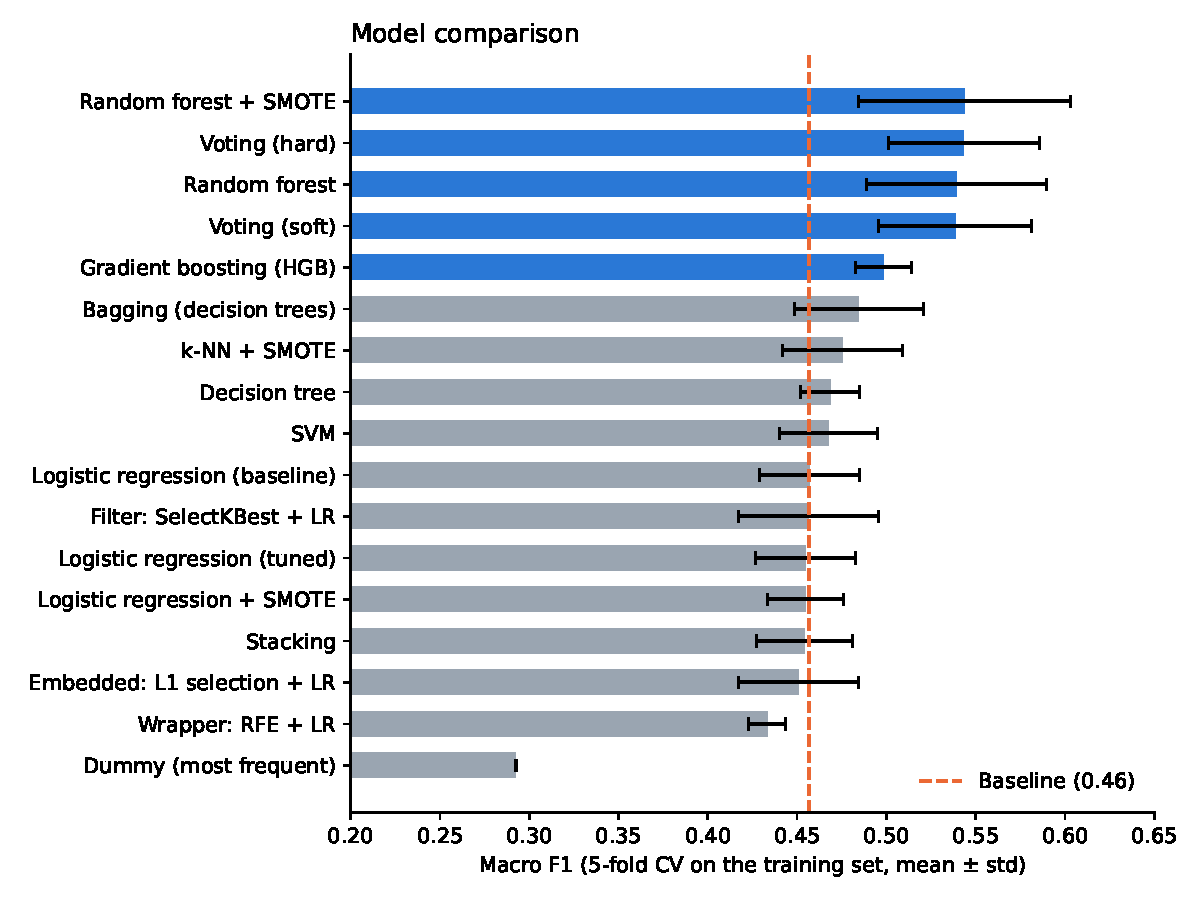
\includegraphics[width=0.75\linewidth]{figures/model_comparison.pdf}
  \caption{Macro F1 of all models (nested 5-fold CV on the training set). Blue: more than 0.03 above the baseline.}
  \label{fig:comparison}
\end{figure}

\textbf{Where the gain comes from.} The out-of-fold predictions (Figure~\ref{fig:oof}) show that the random forest does not find more rare lots than the baseline. The F1 of \texttt{Specialty} goes from 0.64 to 0.82: the baseline sends half of the \texttt{Specialty} lots to the other classes, the forest keeps 79\,\% of them. For \texttt{Commercial}, precision goes up (0.28 to 0.40) but recall goes down (0.64 to 0.51): the baseline flags 331 lots to find 94 sub-grade ones, the forest flags 192 to find 76. For \texttt{Exemplary}, the F1 does not change (0.34 to 0.35). The forest almost never confuses the two extreme classes (3 lots, against 17 for the baseline). In Section~2.1 we said that a lower \texttt{Commercial} recall must be discussed: here it is the price of far fewer false alarms. A buyer who wants to catch every sub-grade lot would still prefer the baseline.

\begin{figure}[h]
  \centering
  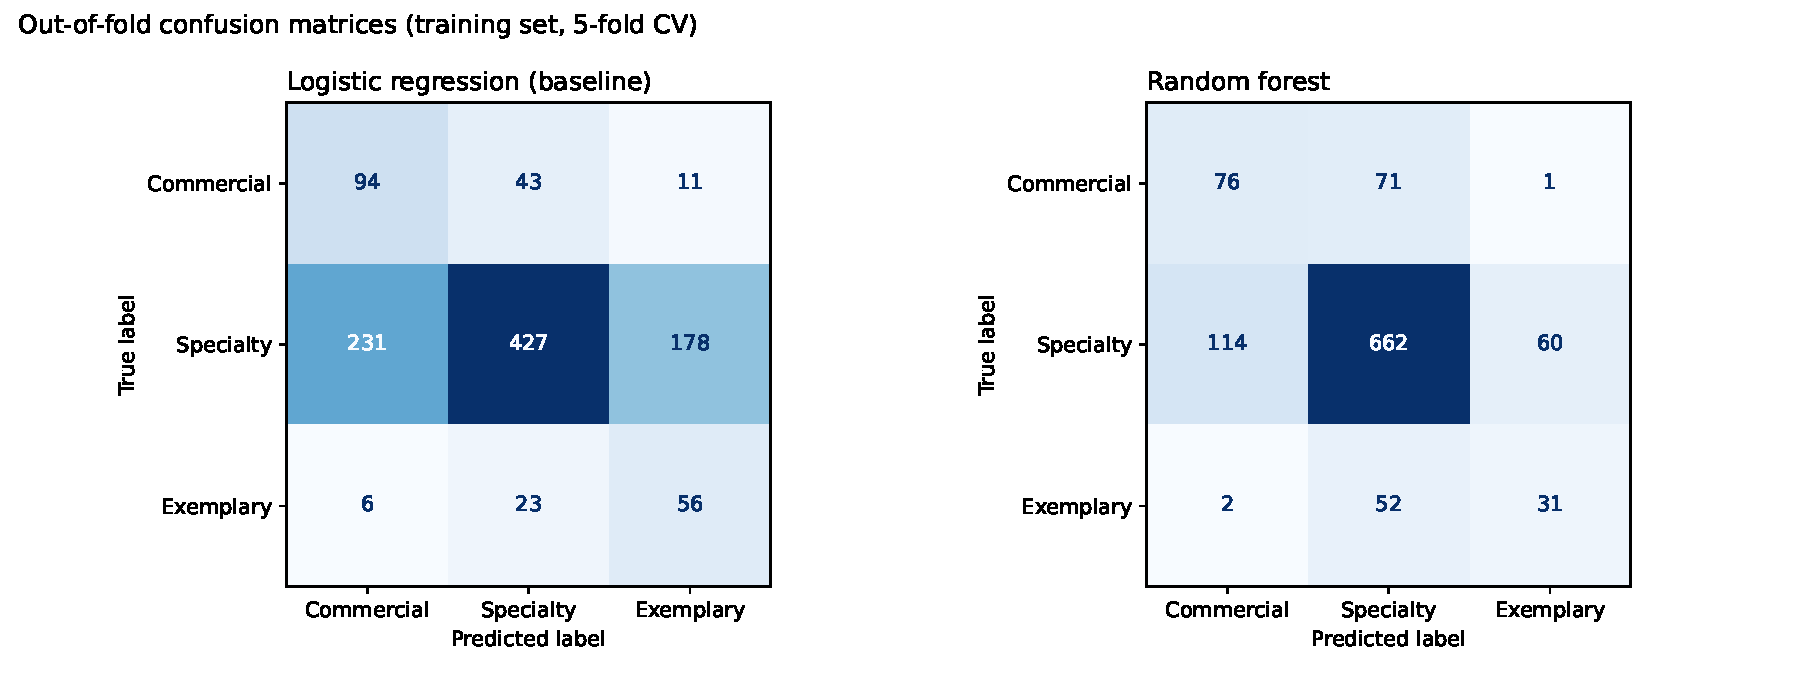
\includegraphics[width=\linewidth]{figures/oof_confusion.pdf}
  \caption{Out-of-fold confusion matrices on the training set (5-fold CV).}
  \label{fig:oof}
\end{figure}

\textbf{Is the gain significant?} The 5 fold scores are not independent (the training folds overlap), so a classic paired t-test underestimates the variance. We use the corrected resampled t-test of \citet{nadeau2003}, on a 5-fold CV repeated 10 times ($J=50$ paired differences, variance multiplied by $1/J + n_{val}/n_{train}$ with $n_{val}/n_{train}=1/4$). The random forest is better by 0.093 macro F1 (corrected 95\,\% confidence interval [0.053, 0.134], $p \approx 3\cdot 10^{-5}$). The test assumes that the differences are roughly normal; Shapiro--Wilk does not reject it ($p=0.39$), and the fallback Wilcoxon test on the 10 repetition means agrees ($p=0.002$). The naive t-test gives $p \approx 10^{-22}$, which shows how much it overstates the evidence.

\textbf{Final model and test set.} We choose the random forest with class weights: it is tied with the best models, it is a single model, and it does not use synthetic data. Its grid search, refit on the whole training set, chooses \texttt{max\_depth=10} and \texttt{min\_samples\_leaf=1}. On the test set, used once, it gets a macro F1 of \textbf{0.63} (95\,\% bootstrap interval [0.55, 0.71]), against 0.52 ([0.45, 0.58]) for the baseline. Both models score higher on the test set than in CV; with only 21 \texttt{Exemplary} and 37 \texttt{Commercial} test lots, a few lots change the score a lot, so the CV value ($\approx 0.54$) remains our best estimate. Our goal from Section~2.1 (CV macro F1 $\geq 0.55$) is close but not reached. The trade-off seen in CV is still there on the test set: \texttt{Commercial} recall 0.68 against 0.78, but precision 0.44 against 0.33.

\textbf{Which features matter?} We measure the permutation importance of each original feature (drop of macro F1 when the feature is shuffled) on the validation folds (Figure~\ref{fig:importance}). Country (0.031) and altitude (0.021) are the main signals, as in the exploration. Category-two defects have a small but stable effect (positive in all 5 folds). \texttt{color} is third on average but uncertain; it is missing much more often for \texttt{Exemplary} lots, so part of its importance may come from how the CQI data was collected, not from the coffee. The years, moisture and region have no measurable effect.

\begin{figure}[h]
  \centering
  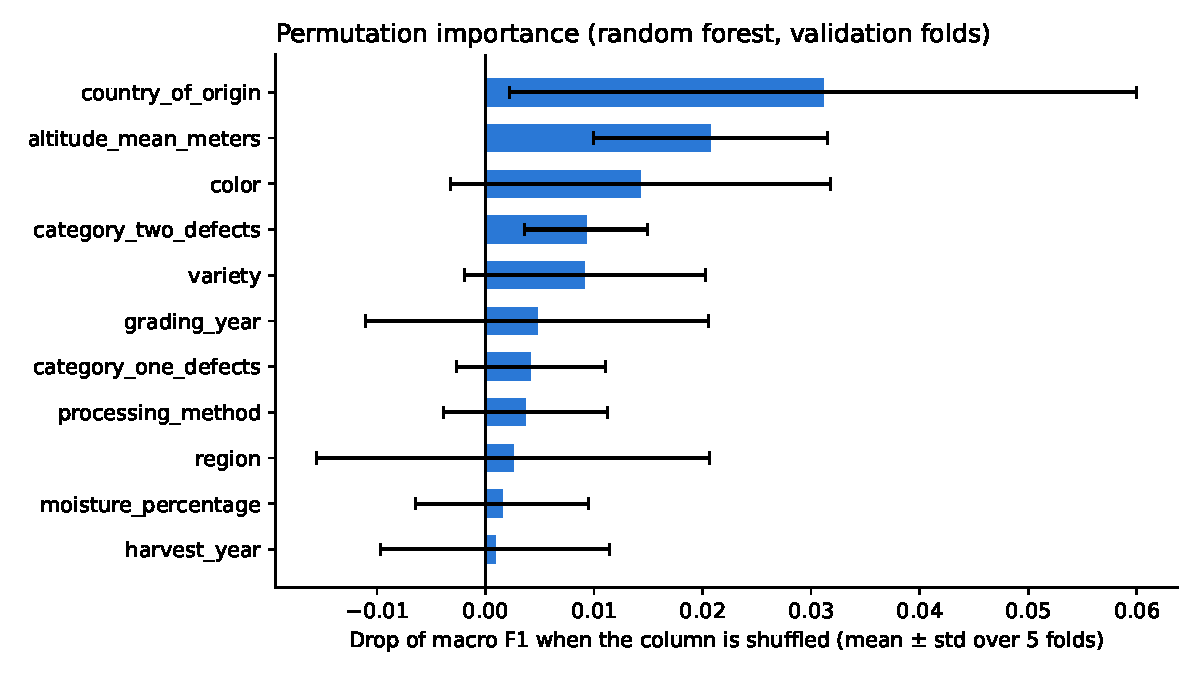
\includegraphics[width=0.75\linewidth]{figures/permutation_importance.pdf}
  \caption{Permutation importance of the final random forest (mean $\pm$ std over the 5 validation folds).}
  \label{fig:importance}
\end{figure}

\textbf{Limits.} The model mainly uses country and altitude: two lots with the same origin but a different work at the farm get almost the same prediction, because the data does not describe this work. Next steps: add the contextual country dataset, tune the decision threshold if a buyer needs a higher \texttt{Commercial} recall, and check the calibration of the predicted probabilities.

\begin{thebibliography}{9}
\bibitem[Cheng(2024)]{cheng2024} Cheng, X. (2024). A comprehensive study of feature selection techniques in machine learning models. \emph{Insights in Computer, Signals and Systems}, 1(1).
\bibitem[Nadeau and Bengio(2003)]{nadeau2003} Nadeau, C. and Bengio, Y. (2003). Inference for the generalization error. \emph{Machine Learning}, 52(3):239--281.
\end{thebibliography}

\end{document}